% !TEX root = main.tex

\section{基本概念}
\subsection{事件与概率}
\begin{proposition}事件的基本运算
	\begin{enumerate}
		\itemsep -3pt
		\item 分配律:$A\cup(B\cap C)=(A\cup B)\cap(A\cup C),\,A\cap(B\cup C)=(A\cap B)\cup(A\cap C)$
		\item 德摩根律:$\overline{A\cup B}=\overline{A}\cap\overline{B},\,\overline{A\cap B}=\overline{A}\cup\overline{B}$
	\end{enumerate}
\end{proposition}
注意概率是对一个集合的函数,有如下定义.
\begin{definition}[概率]
	随机试验$E$的所有可能结果构成$E$的样本空间$\Omega$,$\Omega$的子集称为事件,$\Omega$的幂集构成$E$的事件空间$\mathcal{F}$,记概率函数$\pr{\cdot}:\mathcal{F}\mapsto\rr$满足:
	\begin{enumerate}
		\itemsep -3pt
		\item 非负性:$\pr{A}\geq 0,\forall A\in\mathcal{F}$
		\item 规范性:$\pr{\Omega}=1$
		\item 可列可加性:$A_1,A_2,\ldots$为两两不相容的事件,$\displaystyle \pr{\bigcup_{i=1}^\infty A_i}=\sum_{i=1}^\infty \pr{A_i}$
	\end{enumerate}
\end{definition}
由定义可得概率一些基本性质:
\begin{enumerate}
	\itemsep -3pt
	\item $\pr{\varnothing}=0,\,\pr{A}\leq 1$
	\item 有限可加性:$A_1,A_2,\ldots$两两不相容,$\displaystyle \pr{\bigcup_{i=1}^n A_i}=\sum_{i=1}^n \pr{A_i}$
	\item 若$A\subset B$,则$\pr{B-A}=\pr{B}-\pr{A},\,\pr{B}\geq \pr{A}$
	\item 逆事件概率:$\pr{\overline{A}}=1-\pr{A}$
	\item 容斥原理:
	\[\pr{\bigcup _{{i=1}}^{n}A_{i}}=\sum _{{k=1}}^{n}\left((-1)^{{k-1}}\sum _{\substack{I\subset \{1,\ldots ,n\}\\|I|=k}}\pr{\bigcap _{{i\in I}}A_{i}}\right)\]
\end{enumerate}
\par 本章的重点在于组合计数,正确计算事件数目并套用相应的公式即可.

\subsection{条件概率}
\begin{definition}[条件概率]
设$A,B$为两个事件,且$\pr{A}>0$,则称
\[\pr{B\mid A}=\dfrac{\pr{AB}}{\pr{A}}\]
为在事件$A$发生的条件下事件$B$发生的条件概率
\end{definition}
进而有
\[\prc{B}{A}\pr{A}=\pr{AB}=\prc{A}{B}\pr{B}\]
\begin{theorem}[乘法公式]
设$A_1,A_2,\ldots,A_n$为$n$个事件,$n\geq 2$,且$\pr{A_1A_2\cdots A_{n-1}}>0$,则
\[\pr{A_1A_2\cdots A_{n-1}}=\pr{A_n\mid A_1A_2\cdots A_{n-1}}\pr{A_{n-1}\mid A_1A_2\cdots A_{n-2}}\cdots\pr{A_2\mid A_1}\pr{A_1}\]
\end{theorem}
\begin{definition}[划分]
两两交为空,所有并为全集
\end{definition}
\begin{theorem}[全概率公式]
设试验$E$的样本空间为$S$,$A$为$E$的事件,$B_1,B_2,\ldots,B_n$为$S$的一个划分,且$\pr{B_i}>0$,则
\[\pr{A}=\pr{AB_1}+\pr{AB_2}+\cdots+\pr{AB_n}=\pr{A\mid B_1}\pr{B_1}+\pr{A\mid B_2}+\cdots+\pr{A\mid B_n}\pr{B_n}\]
\end{theorem}
\begin{figure}[H]
\centering
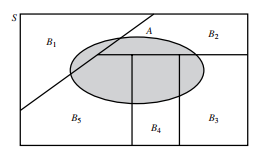
\includegraphics[width=0.35\linewidth]{fig/total_probability.PNG}
\end{figure}
\begin{theorem}[贝叶斯(Bayes)公式]
设试验$E$的样本空间为$S$,$A$为$E$的事件,$B_1,B_2,\ldots,B_n$为$S$的一个划分,且$\pr{A}>0,\pr{B_i}>0$,则
\[\pr{B_i\mid A}=\frac{\pr{B_iA}}{\pr{A}}=\frac{\pr{A\mid B_i}\pr{B_i}}{\displaystyle\sum_{i=1}^nP(A\mid B_i)\pr{B_i}}\]
特别地,当$n=2$时有
\[\prc{B}{A}=\dfrac{\prc{A}{B}\pr{B}}{\prc{A}{B}\pr{B}+\prc{A}{\ol{B}}\pr{\ol{B}}}\]
\end{theorem}
\par 注意贝叶斯公式是用\textbf{先验概率}推\textbf{后验概率}.
\par 在计算条件概率时一定要注意前提条件是什么,并将题设进行转换.
\begin{definition}[独立性]
\rm 对于事件$A_1,\ldots,A_n$,
\begin{itemize}
	\item 若$\pr{A_i\cap A_j}=\pr{A_i}\pr{A_j},\forall\,i,j$,则称$\setenu{A_1}{A_n}$两两(pairwise)独立
	\item 若$\displaystyle\pr{\bigcap_{j\in I}A_j}=\prod_{j\in I}\pr{A_j},\forall I\in 2^{[n]}$,其中$2^{[n]}$为$\{A_i\}_{i=1}^n$的所有子集,则称$\setenu{A_1}{A_n}$相互(mutually)独立
\end{itemize}
\end{definition}
\par 区分以下两个概念
\begin{enumerate}
	\item $A,B$对立(exclusive)/不相容 $\Leftrightarrow \mathbb{P}(A\cap B)=0$,即不相交(disjoint)
	\item $A,B$独立(independent) $\Leftrightarrow \mathbb{P}(A\cap B)=\mathbb{P}(A)\cdot\mathbb{P}(B)$,即不相关(unrelated)
\end{enumerate}